\documentclass{beamer}

\usepackage[utf8]{inputenc}
\usepackage{fancybox}
\usepackage{environ}

\usepackage{tikz}

\beamertemplatenavigationsymbolsempty

\title{1.2 Initial-Value Problems}

\subtitle{a lesson for MATH F302 Differential Equations}

\author{Ed Bueler, Dept.~of Mathematics and Statistics, UAF}

\date{\tiny \today}


\usetheme{Pittsburgh}


\begin{document}

\setbeamertemplate{itemize item}{$\bullet$}
\setbeamertemplate{itemize subitem}{$\circ$}


\begin{frame}
\titlepage

\centerline{\tiny for textbook: \, D. Zill, \emph{A First Course in Differential Equations with Modeling Applications}, 11th ed.}
%\color{green!40!blue}
\end{frame}


\begin{frame}{main purpose of DEs}

\begin{itemize}
\item the main purpose of differential equations (DEs) in science and engineering:

\bigskip

    \centerline{\alert{DEs are models which are capable of prediction}}

\bigskip

\item two things are needed to make a prediction:
\begin{align*}
\begin{matrix}
\text{precise description} \\
\text{of rate of change}
\end{matrix} && \iff && &\text{differential equation} \\
\begin{matrix}
\text{knowledge} \\
\text{of current state}
\end{matrix} && \iff && &\text{initial conditions}
\end{align*}
\item sections 1.1 and 1.2 introduce these two things
\end{itemize}
\end{frame}


\begin{frame}{prediction models}

\begin{itemize}
\item all professionals are skeptics about using math for predictions
\item DEs do \emph{not} ``know the future''
\item \dots but they are \emph{models} which are \emph{capable} of prediction
\item next two slides are examples
\end{itemize}

\bigskip
\begin{quote}
\alert{don't worry}: about understanding the specific equations on the next two slides
\end{quote}
\end{frame}


\begin{frame}{an amazingly-accurate \\ real prediction model}

\begin{columns}
\begin{column}{0.55\textwidth}
\begin{itemize}
\item Newton's theory of gravitation gives remarkably-accurate predictions of planets, satellites, and space probes
\item the DEs at right are Newton's model of many particles interacting by gravity
\item \dots a system of coupled, nonlinear, 2nd-order ODEs for the position $\mathbf{r}_i$ of each object with mass $m_i$
\item adding corrections for relativity makes these predictions practically perfect
\end{itemize}
\end{column}
\begin{column}{0.45\textwidth}
$$\frac{d^2 \mathbf{r}_i}{dt^2} = G \sum_{j\ne i} \frac{m_i m_j}{|\mathbf{r}_j - \mathbf{r}_i|^3} (\mathbf{r}_j - \mathbf{r}_i)$$

\medskip

\quad \tiny \href{https://en.wikipedia.org/wiki/Equations_of_motion}{\texttt{en.wikipedia.org/wiki/Equations\_of\_motion}}
\end{column}
\end{columns}
\end{frame}


\begin{frame}{a pretty-good \\ real prediction model}

\begin{columns}
\begin{column}{0.5\textwidth}
\begin{itemize}
\item \emph{weather prediction} uses Euler's fluid model of the atmosphere
\item \dots a system of PDEs; equations at right
\item predictions have been refined by comparing prediction to what actually happened
\item \dots now we get about 6 days of good/helpful predictions
\end{itemize}
\end{column}
\begin{column}{0.5\textwidth}
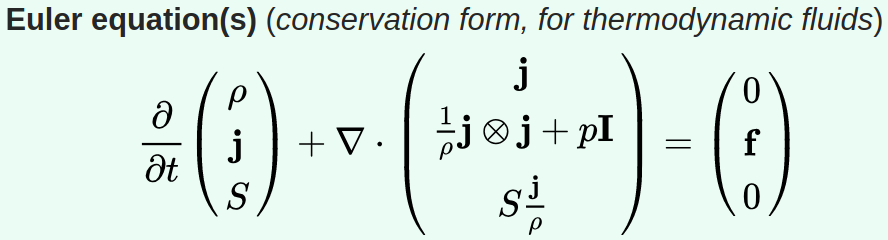
\includegraphics[width=\textwidth]{figs/euler-equations}

\medskip

\quad \tiny \href{https://en.wikipedia.org/wiki/Euler_equations_(fluid_dynamics)}{\texttt{en.wikipedia.org/wiki/}}

\qquad \href{https://en.wikipedia.org/wiki/Euler_equations_(fluid_dynamics)}{\texttt{Euler\_equations\_(fluid\_dynamics)}}
\end{column}
\end{columns}

\bigskip
\begin{quote}
\alert{don't worry}: this course is about ODEs and \emph{not} systems of PDEs
\end{quote}
\end{frame}


\begin{frame}{what kind of student are you?}

\begin{itemize}
\item did you skip the last few slides because you want to know how to do the homework problems quicker?
\item I observe that
    \begin{itemize}
    \item \emph{better} students choose to be curious and interested
    \item \emph{better} students have at least some tentative trust that teachers are seeking an easy path through the whole subject
    \end{itemize}

\bigskip
\item in any case, there \emph{will} be homework about DE models in section 1.3 \dots coming soon
\end{itemize}
\end{frame}


\begin{frame}{example 1}

\begin{itemize}
\item \emph{example}: here is the single most important ODE:
    $$y' = y$$

\vspace{-4mm}
    \begin{itemize}
    \item it is first-order and linear
    \end{itemize}
\item just by thinking you can write down all of its solutions:
    $$y(x) = \hspace{5.0in}$$
\item please graph and label several particular solutions:

\begin{tikzpicture}[scale=1.5]
  \draw[-latex] (-3,0) -- (3,0) node[xshift=2mm] {$x$};
  \draw[-latex] (0,-1) -- (0,1) node[yshift=2mm] {$y$};
\end{tikzpicture}
\end{itemize}

\vfill
\end{frame}


\begin{frame}{example 1, cont.}

\begin{itemize}
\item initial conditions ``pick out'' one prediction (solution) from all the solutions of a differential equation
\item \emph{for example}, fill in the table:

\begin{tabular}{l|l}
ODE IVP & solution \phantom{sldafjdlkajf sd adsfkj asdf} \\ \hline
$y' = y, \, y(0)=3$ & $y(x)=$ \phantom{$\Big|$} \\ \hline
$y' = y, \, y(3)=-1$ & $y(x)=$ \phantom{$\Big|$} \\ \hline
$y' = y, \, y(-1)=1$ & $y(x)=$ \phantom{$\Big|$} \\ \hline
\end{tabular}

\smallskip
\item graph them:

\vspace{-5mm}
\begin{tikzpicture}[scale=1.5]
  \draw[-latex] (-3,0) -- (3,0) node[xshift=2mm] {$x$};
  \draw[-latex] (0,-1) -- (0,1) node[yshift=2mm] {$y$};
\end{tikzpicture}
\end{itemize}

\vfill
\end{frame}

\begin{frame}{example 2}

\begin{itemize}
\item as we will show later,
    $$y(x) = c_1 \sin(3x) + c_2 \cos(3x)$$
is the general solution of ($=$ all of the solutions of)
    $$y'' + 9 y = 0$$
\item \emph{example}.  solve this 2nd-order linear ODE IVP:
    $$y'' + 9y = 0, \quad y(0)=2, \, y'(0)=-1$$
\end{itemize}

\vspace{25mm}
\end{frame}


\begin{frame}{example 3}

\begin{itemize}
\item \emph{example}.  now solve this 2nd-order linear ODE IVP:
    $$y'' + 9y = 0, \quad y(2)=-3, \, y'(2)=0$$
\end{itemize}

\vspace{40mm}
\end{frame}


\begin{frame}{example 4}

\begin{itemize}
\item \emph{example}.  now solve this problem:
    $$y'' + 9y = 0, \quad y(0)=0, \, y(1)=3$$

\vspace{40mm}
\item the above has \emph{boundary} conditions at $x=0$ and $x=1$
    \begin{itemize}
    \item \emph{not} an IVP
    \item potentially problematic; for example, $y'' + 9y = 0, \, y(0)=0, \, y(\pi/3)=3$ has \emph{no} solutions
    \end{itemize}
\end{itemize}
\end{frame}


\begin{frame}{general IVP}

\begin{itemize}
\item in Math 302 we will stick to \emph{initial} conditions
    \begin{itemize}
    \item \emph{not} boundary conditions
    \end{itemize}
\item the general form of an initial-value problem for an ordinary differential equation (ODE IVP):
\begin{align*}
\frac{d^n y}{dx^n} &= f(x,y,y',\dots,y^{(n-1)}) \\
y(x_0) &= y_0 \\
y'(x_0) &= y_1 \\
   &\vdots \\
y^{(n-1)}(x_0) &= y_{n-1}
\end{align*}

\vspace{-1mm}
     \begin{itemize}
     \item this is equation (1) at the start of section 1.2
     \end{itemize}
\end{itemize}
\end{frame}


\begin{frame}{main idea}

\begin{itemize}
\item as suggested earlier, the main idea is that an ODE IVP is a \emph{model capable of prediction}
    \begin{itemize}
    \item law of how things change ($=$ the DE) plus the current state ($=$ the initial values)
    \end{itemize}
\item to have a prediction, two questions need ``yes'' answers:
    \begin{enumerate}
    \item does a solution of the ODE IVP exist?
    \item is there only one solution of ODE IVP?
    \end{enumerate}
\item people often say ``is the solution unique?'' for the second question
\end{itemize}
\end{frame}


\begin{frame}{theorem about main idea}

\begin{itemize}
\item for nicely-behaved first-order ODE IVPs, the answer to both questions is ``yes''!
    \begin{itemize}
    \item ``nicely-behaved'' means that the differential equation is continuous enough
    \end{itemize}
\item consider the first-order ODE IVP
    $$(\ast) \qquad y' = f(x,y), \quad y(x_0) = y_0 \hspace{50mm}$$
\end{itemize}

\begin{theorem}[1.2.1]
Let $R$ be a rectangle in the $xy$ plane that contains $(x_0,y_0)$ in the interior.  Suppose that $f(x,y)$ in $(\ast)$ is continuous and the $\frac{\partial f}{\partial y}(x,y)$ is also continous.  Then there is exactly one solution to ODE IVP, but it may only be defined for a short part of the $x$-axis around $x_0$, i.e.~on an open interval $(x_0-h,x_0+h)$.
\end{theorem}
\end{frame}


\begin{frame}{an example}

\begin{itemize}
\item the last slide was ``mathy''; an example helps give meaning
\item \emph{example}.  verify that both $y(x)=0$ and $y(x)=c x^{3/2}$, for some nonzero $c$, solve the ODE IVP
    $$y' = y^{1/3}, \quad y(0)=0$$

\vspace{30mm}
\item in the above example $\frac{\partial f}{\partial y} = \frac{1}{3} y^{-2/3}$
    \begin{itemize}
        \item it is not continuous on any rectangle around $(0,0)$
    \end{itemize}
\item the theorem on the last slide is true but this example shows you \emph{do} need $f(x,y)$ to be nice
\end{itemize}
\end{frame}


\begin{frame}{conclusion}

\begin{itemize}
\item the main idea of section 1.2 is in this slogan:

\bigskip

\begin{quote}
\alert{if you add initial condition(s) to a differential equation then you can get a single solution}, which can be used to predict
\end{quote}

\bigskip

\item Theorem 1.2.1 says this is actually true of first-order ODE IVPs ($y'=f(x,y)$) with a single initial value ($y(x_0)=y_0$) as long as the function $f$ is nice
\item \emph{important notes}:
    \begin{itemize}
    \item to use the language of prediction, we would call $x<x_0$ the ``past'' and $x>x_0$ the ``future''
    \item for $n$th-order ODEs (second-order, third-order, etc.) the Theorem does not directly apply, but we expect to need $n$ numbers to give adequate initial conditions/values
    \end{itemize}
\end{itemize}
\end{frame}


\begin{frame}{expectations}

\textbf{expectations}:  to learn this material, just watching this video is \emph{not} enough; also
\begin{itemize}
\item \emph{read} section 1.2 in the textbook
\item \emph{do} the WebAssign exercises for section 1.2
\item \emph{think} about these ideas

\bigskip
\item see this page for more on Theorem 1.2.1:

\centerline{\href{https://en.wikipedia.org/wiki/Picard-Lindelof_theorem}{\texttt{en.wikipedia.org/wiki/Picard-Lindel\"of\_theorem}}}
\end{itemize}
\end{frame}


\end{document}

